% For now put all the themes in one file, but split out later as more convenient.
\section{Themes}  \label{sec:themes}


%%%%%%%%%%%%%%%%%%%%%%%%%%%%%%%%%%%%%%%%%%%%%%%%%%%%%%%%%%%%%%%%%%%%%%%%%%%%%%%%%%
%\subsection{Implication of Bayesian philosophy/practices/concepts}  \label{subsec:implications}
%
%[\emph{This may go in section~\ref{subsec:conceptual_issues} instead.}]
%
%\bi
%  \I emphasis of posterior vs.\ minimizing of $\chi^2$
%  \I sampling vs.\ optimization  
%\ei
%
%%%%%%%%%%%%%%%%%%%%%%%%%%%%%%%%%%%%%%%%%%%%%%%%%%%%%%%%%%%%%%%%%%%%%%%%%%%%%%%%%%
\subsection{Likelihood function and Bayes theorem}  \label{subsec:L}

\bi
  \I Recall Bayes theorem introduced (probably) in sec. \ref{subsec:basic_Bayes}
  \I Posing the problem (and the notations): data = model + random error
\beq
y(\gras{x}) = \eta(\gras{x}) + \epsilon
\eeq
with $\eta$ a model that depends on parameters $\gras{x}$, and $\epsilon$ the 
deviation between the output $\eta(\gras{x})$ of the model (a prediction) and 
the experimental data $y(\gras{x})$
  \I Define the likelihood function in both simple (1D) and advanced (ND) case
  \I Everything else follows: GP + MCMC to actually determine $x$, variations on 
     the same theme for model defects ($\epsilon \rightarrow \epsilon + \delta(x)$ 
     and augmented $\chi^2$, choice of prior for $x$, etc.
  \I Example: nuclear forces $\hat{V}_{NN}$, $\hat{V}_{NNN}$, etc., are 
     characterized by a set of parameters $\gras{x} = (x_1, \dots, x_N)$. The 
     predictive power of any quantum many-body method, i.e., of a given model 
     $\eta$, to reproduce nuclear properties $y$ such as masses, radii, 
     separation energies, transition rates, etc., rely on our ability to obtain a 
     reliable parametrization $\gras{x}$ which minimizes the deviation $\epsilon$.
\ei

\begin{figure}[h]
\begin{center}
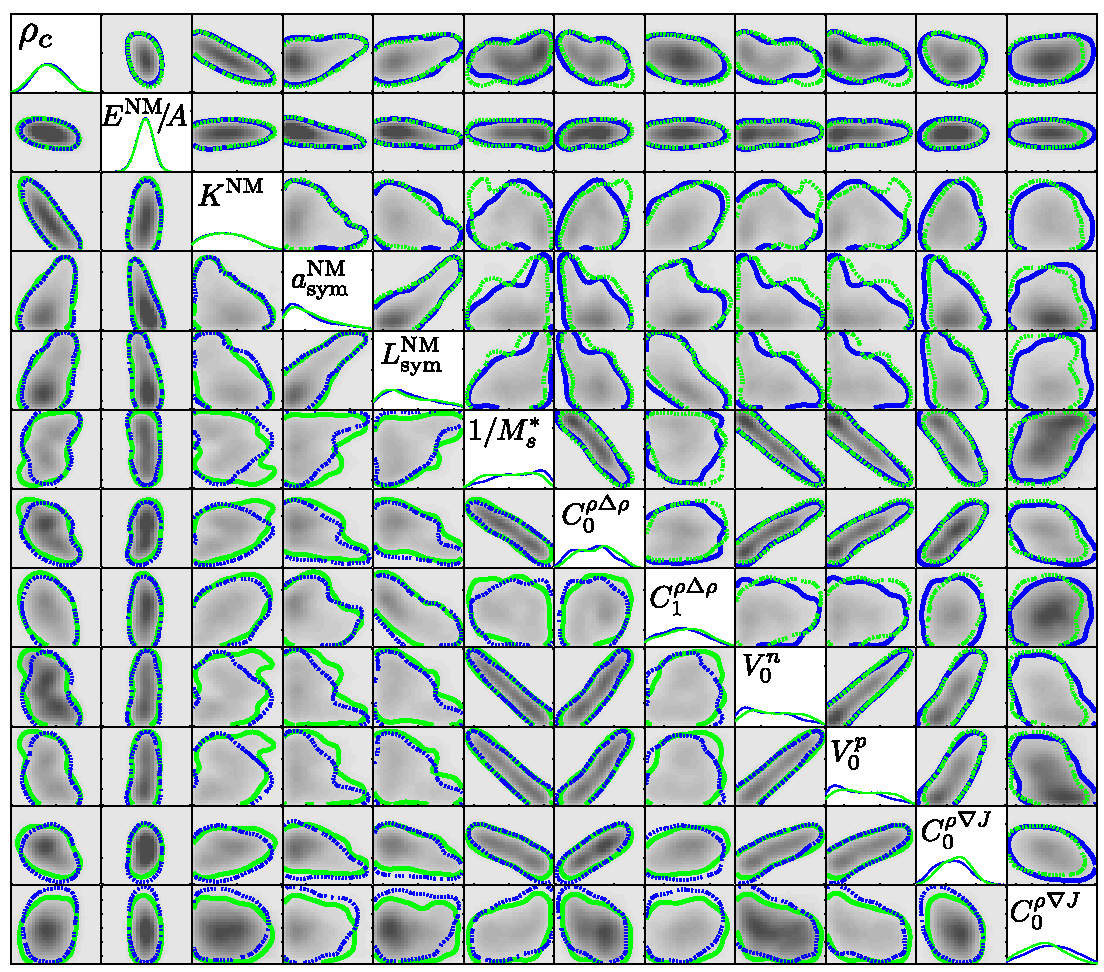
\includegraphics[width=0.6\columnwidth]{figures/UNEDF1_posterior}
\caption{(Color online) Univariate and bivariate marginal estimates of the 
posterior distribution for the 12-dimensional DFT parameter vector of the 
UNEDF1 parameterization of the Skyrme energy functional. The blue lines enclose 
an estimated 95\% region for the posterior distribution found when only the 
original UNEDF1 data are accounted for; the green-outlined regions represent 
the same region for the posterior distribution found when additional data on 
recent mass measurements are also included. For the range of parameter variation, 
see \cite{mcdonnell2015}.
}
\label{fig:UNEDF1_posterior}
\end{center}
\end{figure}

%%%%%%%%%%%%%%%%%%%%%%%%%%%%%%%%%%%%%%%%%%%%%%%%%%%%%%%%%%%%%%%%%%%%%%%%%%%%%%%%%%
\subsection{Gaussian Process (GP) as a tool}  \label{subsec:GP_tool}

\bi
  \I GP simulates correlations between parameters
  \I emulators
  \I discrepant functions / random effects 
  \I linear regression $\rightarrow$ GP
  \I limitations: bad at emulating waveforms (Lackey)
\ei

%%%%%%%%%%%%%%%%%%%%%%%%%%%%%%%%%%%%%%%%%%%%%%%%%%%%%%%%%%%%%%%%%%%%%%%%%%%%%%%%%%
\subsection{Discrepant functions / random effects}  \label{subsec:discrepant}

\bi
  \I Model discrepancy: mock up what we know about the intrinsic limitations of 
     our model into the posterior
  \I data = model + truly random error + systematic bias
  $$ y(x) = \eta(x) + \epsilon + \delta(x) $$
  \I Example of nuclear masses: deviations near closed shells (particle-vibration 
     coupling, pairing phase transition), at $N=Z$ (Wigner energy), in transitional 
     nuclei (shape coexistence) are known but sometimes very hard (=computationally) 
     to model
  \I Using model discrepancies allow ``professional'' fitting of a model at some 
     approximation while resulting parametrization is valid at higher resolution/order.
     Ex.: fit at SR-EDF level, but parameters hopefully valid at MR-EDF
  \I Avoid overfitting
\ei

%%%%%%%%%%%%%%%%%%%%%%%%%%%%%%%%%%%%%%%%%%%%%%%%%%%%%%%%%%%%%%%%%%%%%%%%%%%%%%%%%%
\subsection{\texorpdfstring{$\chi^2$}{chi-squared} and dofs}  \label{subsec:}

   \bi 
       \I $\chi^2/$dof is not meaningful for Bayesian statistics
       \I dofs when there are priors
       \I how should one count dofs?
       \I augmented $\chi^2$: distance from the prior (Bartek's talk?)
       \I When does $\chi^2/$dof make sense?
       \I AWS: Bayes' factors and Occam's razor
   \ei    

%%%%%%%%%%%%%%%%%%%%%%%%%%%%%%%%%%%%%%%%%%%%%%%%%%%%%%%%%%%%%%%%%%%%%%%%%%%%%%%%%%
\subsection{Pitfalls}  \label{subsec:pitfalls}

  \bi
    \I using same data to estimate priors and determine uncertainty
  \ei


%%%%%%%%%%%%%%%%%%%%%%%%%%%%%%%%%%%%%%%%%%%%%%%%%%%%%%%%%%%%%%%%%%%%%%%%%%%%%%%%%%
\subsection{Model selection / comparison (or metrics)}  \label{subsec:model_comparison}

  \bi
    \I laundry list of approaches (see Vera's talk)
    \I new approach for nuclear physics: mixture models (supermodels)
  \ei


%%%%%%%%%%%%%%%%%%%%%%%%%%%%%%%%%%%%%%%%%%%%%%%%%%%%%%%%%%%%%%%%%%%%%%%%%%%%%%%%%%
\subsection{Selection of priors}  \label{subsec:selecting_priors}

  \bi
    \I uniform vs. where it makes a difference
    \I knowledge of underlying model 
    \I running against the boundary
    \I AWS: Jeffrey's priors and invariance with respect to
    parameter transformations
  \ei


%%%%%%%%%%%%%%%%%%%%%%%%%%%%%%%%%%%%%%%%%%%%%%%%%%%%%%%%%%%%%%%%%%%%%%%%%%%%%%%%%%
\subsection{Use of MCMC}  \label{subsec:using_mcmc}

Monte Carlo integration methods are based on the idea that, if one
has a way to generate a random deviate from a probability distribution
defined by the integrand, then one can replace the integral by a sum
(the same formalism applies trivially to multi-dimensional integrals)
\begin{equation}
  \int_a^{b} f(x) dx \approx \frac{\left( b-a\right)}{N} \sum_i p_i 
\end{equation}
where $p_i$ is a list of $N$ random numbers selected from the
probability distribution $f(x)$ with $x \in [a,b]$. Monte
Carlo is typically an efficient method of integration
over direct integration for
problems with large dimensionality. In some cases,
selecting a random deviate from $f(x)$ is not straightforward.
This problem can be handled by importance sampling: one decomposes
$f(x)=g(x)h(x)$ where $g(x)$ is slowly varying with $x$ and $h(x)$
is a function which one can more easily sample random deviates from.

Markov chain Monte Carlo (MCMC) is a type of
importance sampling where one generates random deviates from $h(x)$
by generating a ``Markov chain'', a set of numbers whose distribution
asymptotically approaches $h(x)$. A common approach to generating
a Markov chain is the Metropolis algorithm, but several other methods
exist. The key to the Metropolis algorithm is ergodicity, and this
property guarantees that values in the chain indeed converge to
the desired distributions\footnote{When coding the Metropolis algorithm, we
have found it relatively easy to make subtle errors which violate
ergodicity, so the reader is warned to test their code.}.

Because points in the Metropolis algorithm are often chosen based on a
random step (typically with a fixed maximum step size) from the
previous point, adjacent points in the chain are not statistically
independent. These autocorrelations are the scourge of MCMC methods.
There are two principal methods~\cite{Allen89} for overcoming these
autocorrelations: (i) ``thinning'' the chain and selecting only those
values which are farther apart than the autocorrelation length, and
(ii) block averaging over blocks which have a size larger than the
autocorrelation length. Autocorrelations can often be decreased
by increasing the maximum stepsize, but this comes at a cost of
more Metropolis rejections. The optimal step size is that which
minimizes the computational time between statistically independent
points in the chain~\cite{Sokal80}.

For a one-dimensional function, computing the autocorrelation length
can be done directly using the 
\begin{equation}
  \ell(k) = \frac{1}{\sigma^2(N-k)}
  \sum_i^{N-k} (x_i- \bar{x})(x_{i+k}- \bar{x})
\end{equation}
the autocorrelation length is smallest value of $k$ for which
$\ell(k)$ is zero (within the noise limits set by the size of the data
set). Alternatively, one can use the Kubo formula to
recast the expression... \aws{I will describe the 'acor' method
  here.} For multidimensional functions, it is important to note that
the autocorrelation length of a functions parameters can be wildly
different. In this case, the autocorrelation length of the chain is
the largest autocorrelation length among all of the parameters.

MCMC is particularly useful in Bayesian inference because one is
often required to compute many integrals based on the same kernel,
e.g.
\begin{equation}
  I_1 = \int g_1 h d \vec{x} \quad ; \quad
  I_2 = \int g_2 h d \vec{x} \quad ; \quad \ldots
\end{equation}
where the $g_i$ are slowly varying functions. In this case, MCMC
methods generate a Markov chain for $h$, and then evaluate the
functions $g_i$ for each (statistically independent) element in the
chain. Even if the function $g_1$ is difficult to compute, 
if the functions $g_{i,i\neq 1}$ are easy to compute given the
result of $g_1$, there is a significant time savings to computing
all of the integrals at one time.


  \bi
    \I must be able to evaluate quickly enough
    \I fast model vs. good emulator vs. slow function (dictates what you do)
    \I burn-in as usual; is checking autocorrelation and skipping critical?
    \I nested sampling?
    \I AWS: MCMC pitfalls: Skipping points when the likelihood
    function is zero (bad idea)
  \ei


%%%%%%%%%%%%%%%%%%%%%%%%%%%%%%%%%%%%%%%%%%%%%%%%%%%%%%%%%%%%%%%%%%%%%%%%%%%%%%%%%%
\subsection{Specific issues}  \label{subsec:issues}

  \bi
    \I Instabilities in parameter space
      \bi
        \I undefined $\chi^2$
        \I diagnostics (e.g., response function) 
        \I alternatives?
      \ei     
      \I Bayesian inference for functions rather than for parameters
      \I AWS: Normalization of conditional probabilities?
  \ei

\begin{figure}[h]
\begin{center}
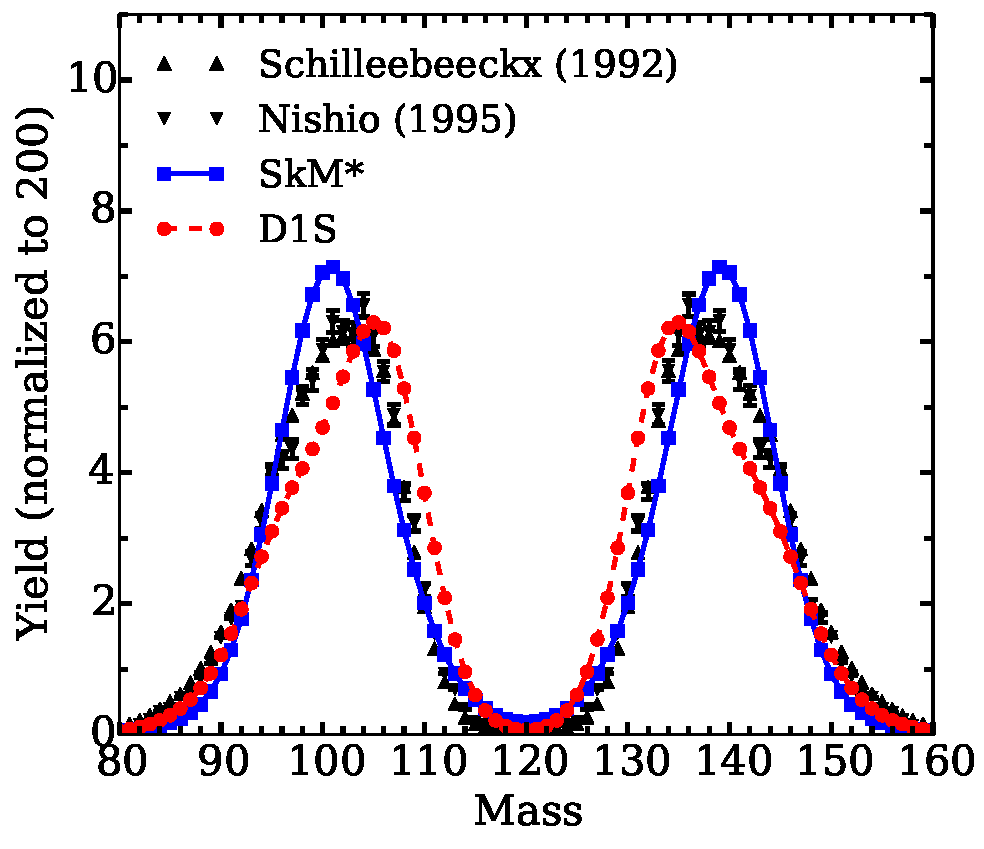
\includegraphics[width=0.6\columnwidth]{figures/fission_yields}
\caption{(Color online) Pre-neutron mass yields for $^{239}$(n,f). The SkM* 
and D1S calculations are compared with two experimental datasets~\cite{schillebeeckx_comparative_1992,nishio_measurement_1995}. The data from 
Nishio are plotted with their statistical uncertainties. Reproduced from \cite{regnier2016}.
}
\label{fig:fission_yields}
\end{center}
\end{figure}


%%%%%%%%%%%%%%%%%%%%%%%%%%%%%%%%%%%%%%%%%%%%%%%%%%%%%%%%%%%%%%%%%%%%%%%%%%%%%%%%%%
\subsection{Understanding of model function}  \label{subsec:model_function}

  \bi
    \I ???
  \ei


%%%%%%%%%%%%%%%%%%%%%%%%%%%%%%%%%%%%%%%%%%%%%%%%%%%%%%%%%%%%%%%%%%%%%%%%%%%%%%%%%%
% \subsection{}  \label{subsec:}
%   \bi
%     \I 
%   \ei

